%

\section{Experiments and Results\label{sec:experiments}}

After presenting the datasets, we provide a parametric study and our results in image classification and retrieval.


\subsection{Experimental settings\label{sec:experimental-settings}}
\paragraph{Base architecture and training settings.}

The convolutional trunk is ResNet-50~\cite{he16resnet}. 
SGD starts with a learning rate of $0.2$ which is reduced tenfold at epochs $30, 60, 90$ for a total of $120$ epochs (a standard setting~\cite{paszke2017automatic}). 
%
The batch size $|\mathcal{B}|$ is set to $512$ and an epoch is defined as a fixed number of $T=5005$ iterations. With uniform batch sampling, one epoch corresponds to two passes over the training set; with RA and $m=3$, one epoch corresponds to $\sim 2/3$ of the images of the training set. 
All classification baselines are trained using this longer schedule for a fair comparison. 

\paragraph{Data augmentation.} We use standard flips, random resized crops~\cite{howard2013some}, random lighting noise and a color jittering of brightness, contrast and saturation~\cite{krizhevsky2012imagenet,howard2013some}. 
We refer to this set of augmentations as ``full'', see details in supplemental~\ref{sec:full-data-augment}. 
As indicated in~\cref{tab:classifres} our network reaches $76.2$\% top-1 validation error under our chosen schedule and data augmentation when trained with cross-entropy alone and uniform batch sampling. 
This figure is on the high end of accuracies reported for the ResNet-50 network~\cite{goyal2017accurate,he16resnet} without specially-crafted regularization terms~\cite{zhang2018mixup} or data augmentations~\cite{cubuk2018autoaugment}. 

%

%
%

%
%
%
%

%

%


\begin{figure}
%
{\small
\begin{minipage}{0.47\columnwidth}
\centering 
Input image \medskip

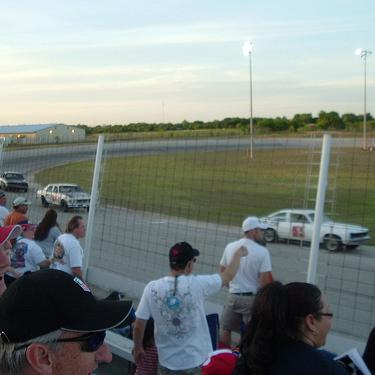
\includegraphics[width=\columnwidth]{figs/per_channel_maps/2/pos.jpg} 

\end{minipage}%
\hfill
%
\begin{minipage}{0.5\columnwidth}
\centering
resolution $s^*=224$ \\

$p^* = 1$ \hspace{1cm} $p^* = 3$ \\

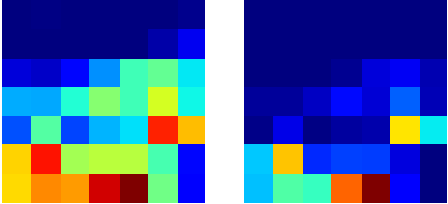
\includegraphics[width=0.8\columnwidth]{figs/per_channel_maps/2/activ_224.pdf}

full resolution \\

$p^* = 1$ \hspace{1cm} $p^* = 3$ \\

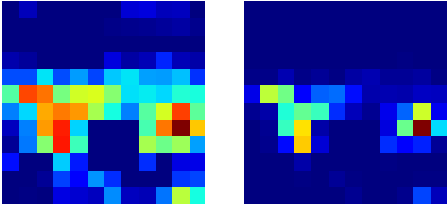
\includegraphics[width=0.8\columnwidth]{figs/per_channel_maps/2/activ_fullres.pdf}
\end{minipage}}
\vspace{-5pt}

\caption{\label{fig:heatmap}
    An off-the-shelf ResNet-50 reacts strongly on channel 909 of the last activation map for class ``racing car''. 
    The image on the left is a hard example for the class.     
    We show channel 909 for that image, at several resolutions and with GeM parameters $p^*=1$ and $p^*=3$.
   	In the low resolution version, the cars are too small to be visible individually on the activation map. 
	In the full resolution version, the location of the cars is more clear. 
	In addition, $p^*$\,$=$\,$3$ reduces the noisy detections relative to the true locations. 
}
\vspace{-7pt}
\end{figure}

%
%

%

%
%
%
%
%
%
%
%

\paragraph{Pooling exponent.} During the end-to-end training of our network, we consider two settings for the pooling exponent in the GeM layer of \cref{sec:p-pooling}: we set either $p=1$ or $p=3$. 
$p=1$ corresponds to average pooling, as used in classification architectures. 
The relevant literature~\cite{radenovic2018fine} and our preliminary experiments on off-the-shelf classification networks suggest that the value $p=3$ improves the retrieval performance on standard benchmarks. 
\Cref{fig:heatmap} illustrates this choice. 
%
%
%
By setting $p=3$, the car is detected with high confidence and without spurious detections. 
Boureau \etal~\cite{Boureau2010ATA} analyse average- and max-pooling of sparse features. 
They find that when the number of pooled features increases, it is beneficial to make them more sparse, which is consistent with the observation we make here. 

%


%

%

\paragraph{Input size and cropping.} As described in~\cref{sec:input-size}, we train our network on crops of size $224\times 224$ pixels.
For testing, we experiment with computing MultiGrain embeddings at resolutions $s^*=224,500,800$. 
For resolution $s^*=224$, we follow the classical image classification protocol ``resolution 224'': the smallest side of an image is resized to $256$ and then a $224\times 224$ central crop is extracted.
For resolution $s^* > 224$, we instead follow the protocol common in image retrieval and resize the largest side of the image to the desired number of pixels and evaluate the network on the rectangular image, without cropping. 

\paragraph{Margin loss and batch sampling.} We use $m$\,$=$\,3 data-augmented repetitions per batch.
We use the default margin loss hyperparameters of~\cite{wu2017sampling} (details in supplementary~\ref{sec:training-hyperparam}). 
As in~\cite{wu2017sampling} the distance-weighted sampling is performed independently on each of the 4 GPUs used for training.

\paragraph{Datasets.} We train our networks on the ImageNet-2012 training set of 1.2 million images labelled into $1,\!000$ object categories~\cite{ILSVRC15}. 
Classification accuracies are reported on the $50,\!000$ validation images of this dataset.
For image retrieval, we report the mean average precision on the {\bf Holidays} dataset~\cite{Jegou2008HammingEA}, with images rotated manually when necessary, as in prior evaluations on this dataset~\cite{Gordo2016DeepIR}. 
We also report the accuracy on the {\bf UKB} object recognition benchmark~\cite{nister2006scalable}, which contains $2,\!550$ instances of objects under $4$ varying viewpoints each; each image is used as a query to find its 4 closest neighbors in embedding space; the number of correct neighbors is averaged across all images, yielding a maximum score of $4$. 
We also report the performance of our network in a copy detection setting, indicating the mean average precision on the ``strong'' subset of the INRIA Copydays dataset~\cite{Douze2009EvaluationOG}.
We add 10K distractor images randomly sampled from the YFCC100M large-scale collection of unlabelled images~\cite{Thomee2016YFCC100MTN}.
We call the combination {\bf C10k}.

The PCA whitening transformations are computed from the features of 20K images from YFCC100M, distinct from the C10k distractors. 

%
%
%

\subsection{Expanding resolution with pooling exponent\label{sec:expand-pooling}}

\begin{figure}
    \centering
    \begin{subfigure}[t]{0.42\columnwidth}
        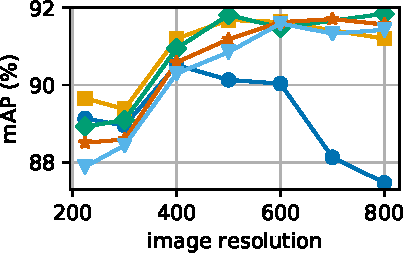
\includegraphics[trim={0.47cm 0 0 0},clip,height=0.7\textwidth]{{{figs/p_plot/p_joint_3B_1.0-holidays}}}
        \vspace{-10pt}
        \caption{Holidays (mAP)}
        \label{fig:p_scale_holidays}
    \end{subfigure}\hfill%
    ~ %
    %
    \begin{subfigure}[t]{0.42\columnwidth}
        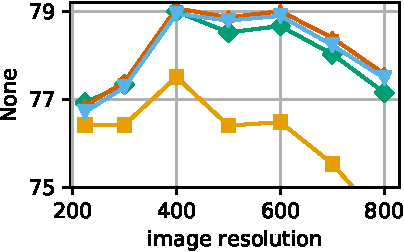
\includegraphics[trim={0.47cm 0 0 0},clip,height=0.7\textwidth]{{{figs/p_plot/p_joint_3B_1.0-classif}}}
        \caption{ImageNet val (top-1)}
        \label{fig:p_scale_classif}
    \end{subfigure}%
%
%
%
%
%
    \begin{subfigure}[t]{0.13\columnwidth}
        ~\hspace{0.2cm}
        \raisebox{0.25in}[0pt][0pt]
        {
\includegraphics[width=\textwidth]{{{figs/p_plot/legend}}}}
    \end{subfigure}%
\vspace{-3pt}
    \caption{\label{fig:p_pooling}
    	Retrieval and classification accuracies as a function of pooling exponent $p^*$ and the image resolution. 
    	At training time, the pooling was $p=3$. %
	Note the clear interaction between the resolution $s^*$ and the pooling exponent~$p^*$. 
    }
\vspace{-5pt}
\end{figure}

As our reference scheme, we train the network at resolution 224x224 with RA sampling and pooling exponent $p=3$. When testing on images with the same 224x224 resolution, this gives a $76.9\%$ top-1 validation accuracy on Imagenet, $0.7$\% points above the non-RA baseline, see \cref{tab:classifres}.

We now feed larger images at test time, \ie, we consider resolutions $s^*$\,$>$\,$224$ and vary the exponents $p^*$\,$\ne$\,$p$\,$=$\,$3$ at test time. 
%
\Cref{fig:p_scale_classif,fig:p_scale_holidays} show the classification accuracy on ImageNet validation and the retrieval accuracy on Holidays at different resolutions, for different values of the test pooling exponent $p^*$. 
As expected, at $s^*$\,=\,$224$, the pooling exponent yielding best accuracy in classification is the exponent with which the network has been trained, $p^*$\,=\,$3$. 
Observe that testing at larger scale requires an exponent $p^*$\,$>$\,$p$, both for classification and for retrieval. 

In the following, we adopt the values obtained by our cross-validation on \inaug, see \cref{sec:expanding-resolution}. 

\subsection{Analysis of the tradeoff parameter \label{sec:tradeoff-parameter}}

%
%
%
%
%
%
%
%

We now analyze the impact of the tradeoff parameter $\lambda$. 
Note, this parameter does not directly reflect the relative importance of the two loss terms during training, since these are not homogeneous: $\lambda$\,=\,0.5 does not mean that they have equal importance. \Cref{fig:gradients} analyzes the actual relative importance of the classification and margin loss terms, by measuring the average norm of the gradient back-propagated through the network at epochs 0 and 120. One can see that $\lambda$\,=\,$0.5$ means that the classification has slightly more weight at the beginning of the training. The classification term becomes dominant at the end of the training, meaning that the network has already learned to cancel data augmentation. 

In terms of performance, $\lambda$\,=$\,0.1$ leads to a poor classification accuracy. 
Interestingly, the classification performance is higher for the intermediate $\lambda$\,=\,$0.5$ ($77.4\%$ at $s^*$\,=\,$224$) than for $\lambda$\,=\,$1$, see \Cref{tab:classifres}. 
Thus, the margin loss leads to a performance gain for the classification task. 
%

%
%

\begin{figure}[t]
\centering
\begin{minipage}{0.5\linewidth}
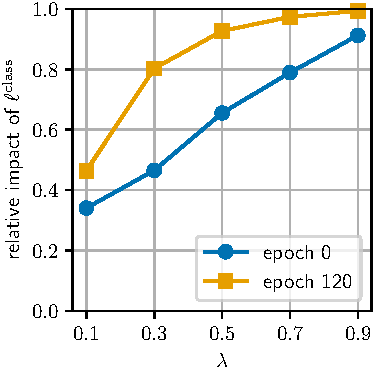
\includegraphics[width=\linewidth]{figs/gradients/gradients}
\end{minipage}
\hfill
\begin{minipage}{0.45\linewidth}
\caption{\label{fig:gradients}
    Fraction of the classification and retrieval terms, measured as $\|g^\mathrm{class}\| / (\|g^\mathrm{class}\| + \|g^\mathrm{retr}\|)$, where the $g^\mathrm{class}$ vector is the gradient from the $\lambda \lclass$ component.
    %
    Note, how the retrieval loss' influence is decreasing over epochs. 
    %
    }
\end{minipage}
\vspace{-5pt}
\end{figure} 


We set $\lambda$\,$=$\,$0.5$ in our following experiments, as it gives the best classification accuracy at the practical resolutions $s^*$\,$=$\,$224$ and $500$ pixels. 
%
As a reference, we also report a few results with $\lambda$\,$=$\,$1$. 
%
%
%

\subsection{Classification results \label{sec:classif-results}}

From now on, our MultiGrain nets are trained at resolution $s$\,=\,$224$ with exponent $p$\,=\,$1$ (standard average pooling) or $p$\,=\,$3$ in the GeM pooling. 
For each evaluation resolutions $s^*$\,=\,$224, 500, 800$, the same exponent $p^*$ is selected according to \cref{sec:expanding-resolution}, yielding a single embedding for classification and for the retrieval. 
%
%
\Cref{tab:classifres} presents the classification results. 
There is a large improvement in classification performance from 
our baseline Resnet-50 with $p$\,=\,$1$, $s$\,=\,$224$, ``full'' data augmentation (76.2\% top-1 accuracy), 
to a MultiGrain model at $p$\,=\,$3$, $\lambda$\,=\,$0.5$, $s$\,=\,$500$ (78.6\% top-1).
We identify four sources for this improvement:
\begin{enumerate}
\item Repeated augmentations: adding RA batch sampling (\cref{sec:data-augmented-batches}) yields an improvement of $+0.6 \%$ $(p$\,$=$\,$1)$.
\item Margin loss: the retrieval loss helps the generalizing effect of data augmentation: $+0.2 \%$ $(p$\,$=$\,$1)$.
\item $p$\,$=$\,$3$ pooling: GeM at training (\cref{sec:p-pooling}) allows the margin loss to have a much stronger effect thanks to increased localization of the features: $+0.4\%$.
\item Expanding resolution: evaluating at resolution $500$ adds $+1.2\%$ to the $p$\,$=$\,$3$ MultiGrain network, reaching the $78.6$ top-1 accuracy. 
This is made possible by the $p$\,$=$\,$3$ training -- which yields sparser features, more generalizable over different resolutions, and by the $p^*$ pooling adaptation -- without it the performance at this resolution is only $78.0\%$.
\end{enumerate}

The $p^*$ selection for evaluation at higher resolutions has its limits: at $800$ pixels, due to the large discrepancy between the training and testing scale for the feature extractor, the accuracy drops to $77.2\%$ ($76.2\%$ without the $p^*$ adaptation).
%

\begin{table}[t]
\centering
\caption{\label{tab:classifres}
	ImageNet 2012 validation performance at top-1~/~top-5 accuracies ($\%$). 
    Resnet-50 is a %
    classification baseline trained with cross-entropy with our training schedule, data augmentation, and uniform batch sampling. 
    MultiGrain uses the same Resnet-50 trunk. 
%
At resolutions $s^*$\,$>$\,224 we evaluate with exponent $p^*$ as described in \cref{sec:expanding-resolution}. %
}
\vspace{-2pt}
{\small
%
%
\begin{tabular*}{\columnwidth}{@{\extracolsep{\fill}}lcccccc}
\toprule
Architecture & $\lambda$ & data & resol. & \multicolumn{2}{c}{train-time pooling}\\ 
& & aug. & $s^*$ & $p = 1$ & $p = 3$ \\
\midrule

ResNet-50  & & full & $224$ & $76.2$ / $92.9$ & $76.2$ / $93.1$\\
MultiGrain & $1$ & full & $224$ & $76.8$ / $93.2$ & $76.9$ / $93.5$ \\
MultiGrain & $0.5$ & full & $224$ & $77.0$ / $93.6$ & $\bm{77.4}$ / $\bm{93.6}$ \\
MultiGrain & $0.5$ & AA & $224$ & $77.4$ / $93.6$ & $\bm{78.2}$ / $\bm{93.9}$ \\
MultiGrain & $0.5$ & full & $500$ & $76.5$ / $93.5$ & $\bm{78.6}$ / $\bm{94.4}$ \\
MultiGrain & $0.5$ & AA & $500$ & $77.7$ / $94.0$ & $\bm{79.4}$ / $\bm{94.8}$ \\
MultiGrain & $0.5$ & full & $800$ & $73.5$ / $93.5$ & $77.2$ / $93.5$ \\
MultiGrain & $0.5$ & AA & $800$ & $74.1$ / $91.8$ & $77.8$ / $93.9$ \\
\midrule
\multicolumn{3}{l}{PyTorch model zoo} & $224$ & $76.1$ / $92.9$ \\
\multicolumn{3}{l}{mixup~\cite{zhang2018mixup}} & $224$ & $76.7$ / $94.4$ \\
\multicolumn{3}{l}{BA ($|\mathcal{B}| = 1024$)~\cite{2019arXiv190109335H}} & $224$ & $76.9$ / \makebox[\widthof{$94.5$}][c]{--} \\
\multicolumn{3}{l}{AutoAugment~\cite{cubuk2018autoaugment}} & $224$ & $77.6$ / $93.8$ \\
\bottomrule
\end{tabular*}

%
%
%

%
%
%
%
%
%
%
%
%
%
%}
\vspace{-2pt}
\end{table}

\paragraph{AutoAugment}~\cite{cubuk2018autoaugment} (AA) is a method to learn data-augmentation  
%
%
%
%
using reinforcement learning techniques to improve the accuracy of classification networks on ImageNet. 
We %
directly integrate the data-augmentations found by the algorithm 
\cite{cubuk2018autoaugment} trained on their Resnet-50 model using a long schedule of 270 passes over the dataset, with batch size $4096$. 
We have observed that this longer training gives more impact to the AA-generated augmentations. 
We therefore use a longer schedule of 7508 iterations per epoch, keeping the batch size to $|\mathcal{B}|=512$. 

Our method benefits from this data-augmentation: 
MultiGrain reaches $78.2\%$ top-1 accuracy at resolution $224$ with $p$\,$=$\,3, $\lambda$\,$=$\,0.5.
To the best of our knowledge, this is the best top-1 accuracy reported for Resnet-50 when training and evaluating at this resolution, significantly higher than the $77.6\%$ reported with AutoAugment alone~\cite{cubuk2018autoaugment} or $76.7\%$ for mixup~\cite{zhang2018mixup}.
Using a higher resolution at test time improves the accuracy further: we obtain $79.4\%$ top-1 accuracy at resolution $500$. 
Our strategy of adapting the pooling exponent to a larger resolution is still effective, and significantly outperforms the state of the art performance for a ResNet-50 learned on ImageNet at training resolution $224$. %



%
%
%
%
%
%

%
%
%
%
%
%


%
%

%
%

\begin{table}
\centering
\caption{\label{tab:instanceres}
	Instance search results and baselines, on Holidays ($\%$~mAP) and UKB ($/4$).
	We set $p=3$ pooling at training time for our MultiGrain models, and $p^*$ set as given in \cref{sec:expanding-resolution}. 
	$\dagger${\small \em GeM is fine-tuned at resolution 362x362 on additional images tailored to the retrieval task. Their best result is obtained with multi-scale input and implies additional processing.
}}
\vspace{-2pt}
%


%
%
%
%
%
%
%
%
%
%
%
%
%
%
%
%
%
%
%
%
%
%
%
%
%
%
%
%

\def \mysp {\hspace{3pt}}
{\small
%
\begin{tabular}{@{\hspace{5pt}}l@{\hspace{5pt}}r ccc@{\hspace{5pt}}}
\toprule
Method & resol. $s^*$ & Holidays & UKB & CD10k \\ 
%
\midrule
MultiGrain $\lambda=1$                     & 500  & {\bf 91.8} & 3.89       & {\bf 81.1} \\
MultiGrain $\lambda=1$                     & 800  & 91.6       & {\bf 3.91} & {\bf 82.5} \\
MultiGrain $\lambda=0.5$                   & 500  & 91.5       & {\bf 3.90} & 80.7 \\
MultiGrain $\lambda=0.5$                   & 800  & {\bf 92.5} & {\bf 3.91} & 78.6 \\
\hline 
%
Fisher vectors~\cite{jegou2012aggregating} & 800  & 63.4       & 3.35       & 42.7 \\
Neural codes~\cite{babenko2014neural}      & 224  & 79.3       & 3.56 \\
ResNet-50 RMAC~\cite{Gordo2016DeepIR}      & 724  & 90.9  \\
ResNet-50 RMAC~\cite{Gordo2016DeepIR}      & 1024 & 93.3 \\
ResNet-101 RMAC~\cite{Gordo2017EndtoEndLO} & 800  & 91.4 & 3.89\\
GeM$^\dagger$~\cite{radenovic2018fine}     & {\bf 1024} &  {\bf 93.9} \\
\bottomrule
\end{tabular}
}
\vspace{-5pt}
\end{table}

\subsection{Retrieval results \label{sec:retrieval-results}}

We present our retrieval results in \cref{tab:instanceres}, with an ablation study and copy-detection results in the supplemental material (\ref{sec:ablationretrieval}). 
Our MultiGrain nets improve accuracies on all datasets with respect to the Resnet-50 baseline for comparable resolutions. 
Repeated augmentations (RA) is again a key ingredient in this context.

We compare with baselines where no annotated retrieval dataset is used. 
\cite{Gordo2016DeepIR,Gordo2017EndtoEndLO} give off-the-shelf network accuracies with R-MAC pooling. 
MultiGrain compares favorably with their results at a comparable resolution ($s^*$\,$=$800). 
They reach accuracies above $93\%$ mAP on Holidays but this requires a resolution $s$\,$\ge$\,1000 pixels. %

It is also worth noting that we reach reasonable retrieval performance at resolution $s^*$\,$=$\,500, which is a interesting operating point with respect to the traditional inference resolutions $s$\,$=$\,$800$--$1000$ for retrieval. 
Indeed, a forward pass of Resnet-50 on 16 processor cores takes $3.80$s at resolution $500$, against $18.9$s at resolution $1024$ ($5\times$ slower).
%
Because of this quadratic increase in timing, and the single embedding computed by MultiGrain, our solution is particularly adapted to large-scale or low-resource vision applications.

For comparison, we also report some older related results on the UKB and C10k datasets, that are not competitive with MultiGrain. 
Neural codes~\cite{babenko2014neural} is one of the first works on retrieval with deep features. 
The Fisher vector~\cite{jegou2012aggregating} is a pooling method that uses local SIFT descriptors. 

At resolutions $500$ we see that the results with the margin loss ($\lambda$\,$=$\,0.5) are slightly lower than without ($\lambda$\,$=$1). 
This is partly due to the limited transfer from the \inaug task to the variations observed in retrieval datasets. 

%

%
%
%



%
%
%
%
%
%
%
%

%
%
%
%
%

%
%

%


